\section{Real Time Pricing for Charging Electric Vehicles}
The restructuring of the electric grid over the last decade has lead to the introduction of new pricing schemes.  Traditionally, users were given one flat rate for the cummulative electricity consumed during any given month.  Now, utilities have begun to offer programs such as two-tier pricing, in which a more expensive price is given to consumption mid-day, and in the summer.  This scheme helps send pricing signals to the consumers, which had never previously been done.  While the two-tier system may send better signals than the single rate, the real time price is volatile and hard to represent.  This leads to improper signals reaching the consumer.  When the consumer is able to time-shift demand, a suboptimal demand schedule is likely.  When the consumer is able to arbitrage, the utility will be exposing itself to losses, which are then recovered through the rate base.  Also, the optimal charging or arbitrage schedule is never obtained, leading to deadweight loss in the system.

This paper starts with an introduction to power systems and the wholesale electricity market.  It will explain how real time prices are decided and the utilties' role in distribution to consumers.  Then, an introduction into modern electric vehicles will be given.  These represent a new, significant load to utilties and the grid.  They are also flexible in their charging schedules, leading to the ability to time-shift demand.  As the battery technology improves, arbitrage on time-varying pricing will become more prevalent.  Time-shifting demand and arbitrage will be explained in the context of an electric vehicle operating on a power system with a wholesale electricity market.  The interaction between the pricing schemes of utilities and the operation of electric vehicles will be explored from the perspective of the utility and the consumer.  Finally, the conclusion that real time pricing is better for electric vehicle loads will be drawn.


\subsection{Power Systems}
	
A power system is divided into 3 primary systems; power generation, transmission, and distribution to load.  The bulk power system for the United States runs on alternating current at 60$hz$.  At any given point in time, power is injected into the system at generator assets and withdrawn from the system at areas of demand.  The net power injections at each location along with the physical characteristics of the power lines uniquely determine where the electricity flows on the transmission system.  Due to this, it is impossible to decide how much power flows on each power line; it is determined by physical laws.  The power flows can only be changed by changing the net power injects at each of the nodes.  Also, energy losses due to resistance of power flow heat up the transmission line.  This leads to problems such as sagging and possibly outage of the line.  Thus it is required to keep the power flow on lines within certain constraints.  

Recently, the market has been restructured to allow competition in the power generation sector.  In order to do this, Independent System Operators (ISO) were formed to operate the power grid.  These are typically non-profit entities regulated by the Federal Energy Regulatory Commission.  The ISO's job is to determine the amount of power each generating asset produces to keep the transmission system within its limits and provide energy, within its region, at the lowest cost.  

\subsubsection{Wholesale Electricity Markets}

The major transmission networks in North America are currently divided into ten ISOs which run the wholesale electricity markets across the country.  The Midwest Independent System Operator (MISO) is the designated ISO for the Midwest United States and Maintoba, Canada, which began market operation in 2005.  In 2011, the value of the real time load cleared was \$18 billion.  This money is dispersed to generating assets, transmission improvements, wind integration, long term planning, and to run MISO.  The pricing scenarios used in this paper will be taken from MISO's market data.  MISO's mission is to ensure reliable, least-cost delivered electricity for consumers.	  

In order to perform this job, the ISO uses 3 primary markets for determining how much each generator should produce at any given time.  The first market is bi-lateral contracts.  These are long term contracts between producers and suppliers to exchange a certain quantity of energy at a given price.  These contracts help provide reliable, long term forecasting for supply and load, which reduces exposure to the volatility of the day ahead and real time markets.  

The day ahead market takes bids from generators which contain an array of costs to produce a certain amount of electricity.  The generators also provide additional constraints which they need to operate within, such as ramping rates and start-up and shut-down times and costs.  In addition to generators information, forecasts for demand of the following day will be used to get an estimate of the amount of generation needed.  Using the transmission constraints for the given network, the ISO will clear this market during the previous day.  This process usually takes around 4 hours and is done with specialized optimization tools solving the optimal power flow problem with security constraints.  The outcome of this process is hourly prices, locational marginal prices (LMP), at each location in the network for the following day.  These prices are guaranteed and any deviation from the schedule will need to be made up in the real-time market.	

The real-time market makes up for errors in forecasting as well as possible outages in generation or transmission.  This market operates on 5 minute intervals and can be extremely volatile.  Similar methods are used to clear this market, although simplified due to the time constraint.  Price spikes can occur during times of peak demand and a congested grid, in which the price of electricity can become over 10-20 times as expensive.  The reverse is also possible, during times of low demand it is possible for negative prices on the real time market.  This occurs because the generators are constrained by ramping rates and there is too much production on the grid. In figure (\ref{fig:lmpmiso}), there are negative prices across the Midwest and in particular Iowa with much higher prices in Illinois.  This LMP snapshot is taken at night when there is low demand for electricity as well as increased production from wind farms located in the Midwest.  The differences in prices suggest a transmission constraint between the Upper Midwest and Illinois.    


\begin{figure}
\centering
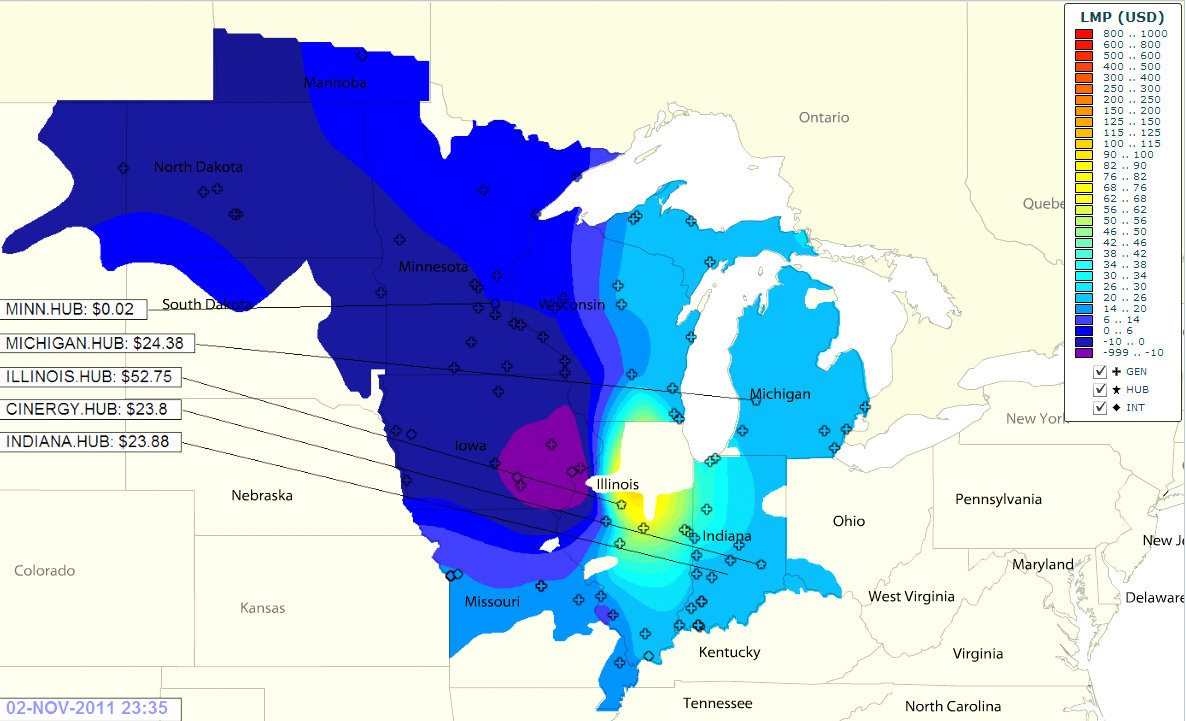
\includegraphics[width=5in]{lmp}  
\caption{Location Marginal Prices (LMP) for Midwest ISO's territory}
\label{fig:lmpmiso}
\end{figure}

\subsubsection{Electric Utilities}
In the modern electricty system, electric utilities are primarly responsible for distribution of electricity to consumers within their territory.  Utilities have retained some of their generating assets, but will typically buy from wholesale markets to meet consumer demand.  Madison Gas and Electric (MG\&E) is the primary electric utility for in and around Madison.  In 2012, around 38\% of electricity sold to consumers has been sourced through the open market.  Traditionally, at the end of every month, Utilities will count how much electricity was consumed and charge a single rate.  This single rate prevents consumers from seeing the price signals that Utilities are facing for their marginal cost of electricity.  In order to improve this situation, Utilities have begun offering market based programs to reduce the cost of peak electricty demand.  These programs include two-tier pricing, real time pricing, cut-off rates, and demand response programs.  

	Two-tier pricing sets up two time periods throughout the day that are charged different rates for the electricity consumed.  MG\&E current rates are 23c and 4c for on-peak and off-peak in summer and 20c and 4c for winter, where on-peak is defined as 10 am to 9 pm Monday through Friday.  Real time pricing gives consumers varying prices over short time intervals, such as an hour.  These prices would be above the marginal cost of grid electricity, allowing for the utility to earn its regulated profit for serving consumers.  Cut-off rates give the utility the ability to cut back certain loads in response to a peak demand situation.  In return, the consumer recieves a better price on electricity.  Demand response programs allow negative demand to be bid into the ISO's markets.  If these bids clear the market, the consumer will have to reduce their demand by the given amount and recieve the bid price.  

\subsection{Electric Vehicles}
Electric vehicles and plug-in hybrids have been starting to fill a role in today's transportation market.  In 2011, around 18,000 plug-ins were sold in the United States.  These vehicles are driven by an electric power train, versus the standard internal combustion engine.  An electric power train consists of electric motors for each wheel, an energy storage system, a controller, and a charging system.  Electric motors are around 90\% efficient converting energy to propulsive power and can also be used in reverse as a generator.  This latter situation is useful for regenerative braking, in which instead of transforming the kinetic energy of the moving car into heat, it is recaptured and stored.  The controller is responsible for operation of the motor and storage system so that the vehicle behaves in a comfortable manner for the user.  The energy storage system is a stack of lithium-ion batteries, typically sized to allow for a given range of travel.  The charging system is extremely important to perserving the life of the batteries as well as providing the user with flexible operation.  

\subsubsection{Energy Storage and Time-Varying Prices}
Energy storage offers considerable flexibility for an electric power system.  Currently, without any cost-effective, large form of storage, the demand for electricity has to be met instaneously by the supply.  Because the demand is variable and uncertain, the suppliers need to be able to quickly respond to changes in demand.  The ramping rate is the most distinguishing characteristic of generating assets.  Generating assets are typically divided into two primary classes, baseload power and peaking power.  Baseload power has slow ramping rates, but low costs.  Examples of baseload power are coal and nuclear power plants.  Peaking power has fast ramping rates, but high cost.  The main peaking plant is a natural gas power plant, but hydro-electric power can also serve the role.  The interaction of variable demand, transmission congestion, and generating assets across the cost/ramping rate spectrum lead to time-varying electricity prices.    

\subsubsection{Quick Charging}
Using a standard 110v plug-in system, it can take 12-24 hours to charge the batteries.  This can be a problem for people who want to use their car.  	In order to increase the charging rate, a higher voltage can be used.  For home charging, a 220v system is typically used which can charge reasonable sized battery stacks in a few hours.  However, it is possible to use 440v or even 880v systems with various power electronic components to achieve charging times on the order of 30 minutes to an hour.  These new charging systems will become important to allow for the flexibility people expect from their vehicles.  However, these fast charging systems place increase stress on the batteries and have been shown to degrade their life.  Also, these systems can put tremendous stress on the grid by adding a new, significant load.  Transmission and distribution systems will have to be upgraded as electric vehicles become an increasing share of the automobile market.    


\subsection{Time-Shifting Demand and Arbitrage}
The demand for energy from an electric vehicle is more flexible than other demands.  Vehicles often spend more than half of their time sitting in a stall waiting to be used.  This allows charging systems to time-shift the loading profile, while still meeting the consumers' traveling constraints.  However, with a single rate pricing scheme, there is no motivation to time-shift demand.

The ability to store energy and dispatch it creates an arbitrage opportunity on the time-varying price of electricity.  Arbitrage is the process of taking advantage of price differences in different markets.  Here, the different markets are simply the points in time during the day, at which each point must have a supply of electricity greater than demand.  The demand for electricity has both daily and seasonal variation.  The price of electricity tends to be low during the night and winter and high during the day and particularly summer.  To engage in arbitrage over the daily variation of electricity prices, one would store energy during the night when the prices are low and then sell during the day when the prices are high.  

There are two forms of arbitrage availble based on the electricity markets.  The first type is a risk-free arbitrage that earns a profit and no possibility of negative cash flows by operating strictly on the day-ahead market.  The other type is a statistical arbitrage which utilizes the day-ahead and real-time market and refers to a positive expected profit.    

\subsection{Utilities and Electric Vehicles}
As electric vehicles are introduced to the grid, the utilties are faced with the task of providing energy to power these vehicles.  The utility has to decide what the pricing options are to consumers who wish to use electric vehicles.  Using a charging model for electric vehicles, a single rate, a two-tier rate, and real time pricing model will be evaluated.  The consumer will recieve the given pricing scheme while the utility can always buy and sell to the grid at market price.  This charging model will be used to look at the problem from the perspective of the consumer and the utility.

\subsection{Charging Model}
The charging model is used to operate an electric vehicle on a wholesale power system.  The model uses a distribution of possible travel schedules to ensure the consumer is able to meet all of its travel needs.  The model allows for both a day-ahead market and a real-time market for electricity and allows for arbitrage or just time-shifting demand.  Its objective is to maximize profit or minimize cost while meeting the travel needs of the user.  This model does not take into account charging preferences, such as plugging in the car once home from work.  The reason for excluding this behavior is because a controller can be designed to optimize the charging times with no loss of convenience to the end user.  The market prices are MG\&E's electricity prices for Madison, Wisconsin from MISO's historic data.  The single tier and two-tier rates are the rates prescribed by MG\&E for residential customers.  The parameters for the storage system are based off plug-in electric vehicles of the Nissan Leaf and Tesla Model S.  The full charging model can be found in appendix (\ref{charge}).

The travel schedule used represents around 60 miles per day of driving throughout the working week.  The results shown for the following sections will be average daily costs of using a Tesla Model S to meet this travel demand.  To compare this to a traditional compact car that gets 30 mpg, the average cost per day would be around \$7.48, at the current rate of \$3.74 for gasoline in Wisconsin.

\subsubsection{Single Rate}
Since the model only accounts for pricing and no charging preferences, all of the charging schedules are optimal.  Also, since there is only one pricing rate, no arbitrage is possible.  Altough the consumer's charging profiles are all optimal, the utilities' cost for electricity need not be optimal.  

The average cost for the consumer to charge the vehicle is around \$3.81.  The cost the utility pays will depend on the specific charging schedule used, which are all optimal to the consumer in a single tier system.  The range of costs to the utility in this situation is between 51c and \$1.20.

\subsubsection{Two-Tier Rate}
The optimal charging schedule for the two-tier rate is to charge during off-peak and if arbitrage is allowed, sell during on-peak.  This still allows for considerable flexibility for the charging schedule while staying optimal to the consumer.  It also opens up arbitrage opportunities that are not possible with the single rate system.  The results for no arbitrage allowed will be presented first, followed by allowing arbitrage.

In the situation with only time-shifting demand, the average cost to the consumer is \$1.27.  This savings to the consumer comes mostly from the profits to the utility in the single rate scenario, since the cost to the utility remains similar at 52c to \$1.04.  One interesting note is that the range of costs to the utility has shrunk, removing the worst case cost scenarios.

By allowing for arbitrage, the consumer can engage in guaranteed arbitrage between the off-peak and on-peak prices.  Now, instead of paying to operate the vehicle, the arbitrage is able to pay for the needed electricity as well as make a profit.  The average profit per weekday for the consumer is \$9.36.  If the utility is lucky, the charging schedule can align nicely with the real time prices, giving the utility a profit of \$2.03.  However, the utility must now pay the consumer the \$9.36, leaving the utility at a net loss of around \$7.34.  If the utility is unlucky, the cost of the charging schedule based on grid prices is \$1.53.  The net cost to the utility is \$10.89.  As can be seen, the two-tier rate system does not properly convey price signals to the consumer when arbitrage is allowed.

\subsubsection{Real Time Pricing}
The real time pricing system gives the consumer hourly price signals throughout the day.  The consumer can purchase the electricity at a premium over what MG\&E pays for the electricity and also sell electricity back to MG\&E at the market price.  This allows the utility to continue earning a profit and sends the proper price signals to the end user.

Using just time-shifting demand, the average cost for using the electric vehicle in the real time pricing scenario is 89c.  Now, the interests of the consumer directly align with that of the utility, and there is no longer a range of costs to the utility.  In this situation, the utilities' average cost for this electricty is 45c.  Since 45c is the lowest average cost of supplying this electricity, this situation has the largest total surplus out of all the pricing schemes.  Also, distribution between utility and consumer can be easily changed without perverting the price signals by adjusting the price premium to the consumer.  Here, the price premium was 100\% over grid price.

Now, allowing for arbitrage, the consumer earns a profit of 29c per day after paying for the electricity needed for driving.  At the same time, the utility earns a profit of \$1.02.  Now that the price signal of the consumer aligns with that of the utility, the arbitrage opportunity is profitable for both parties.


\subsection{Conclusion}

As utilities begin to integrate electric vehicles into the grid, it will be critical that proper price signals are sent to consumers.  Even with just time-shifting demand, utilities can end up at the short end of the stick and the consumers still have to pay more for electricity in the two-tier system.  By giving the consumer the proper price signals, both parties minimze cost when the consumer uses the optimal choice.  Additionally, the two-tier pricing system seems to be dissadvantagous to utilities when the consumer can easily time-shift demand.  These losses to the utility are then recovered through an increase in the rate base, that is raising the single and two-tier prices.  The only real savings in the system going from the single rate to the two tier rate is the reduction in the actual cost of the grid prices.  The upper bound of cost in the two tier rate was \$1.04, compared to the \$1.20 in the single tier system.  This comes at a significant cost of two-tier metering infrastructure and operate cost.  If the utility moves straight to real time pricing, the true cost of electricity goes from a range of 52c to \$1.04 to a cost of 44c.  Now, instead of just decreasing the upper bound of cost, the optimal charging schedule for the consumer is exactly the same as that of the utility, which ensures a reduction in total cost for everyone who participates in the system.

\subsection{The Charging Model for Electric Vehicles}
\label{charge}
This model schedules a charging profile on the day ahead market and operates the storage system on the real time market.  The optimal solution is based upon the day ahead prices and a distribution of possible travel schedules and real time prices.  


\subsubsection{The Mathematical Formulation}
A mathematical model of this problem will be developed to schedule the charging profile on the day-ahead market and then operate the storage system on the real time market.  Let $\cT = \left\{ 1, 2, \cdots, 24 \right\}$ be the 24 hours in a day.  Also, let $e_t$ be the level of the storage system at time $t$, $s_t$ be the amount of energy stored, and $d_t$ be the amount of energy dispatched.  With $\eta$ being the round trip efficiency, the following represents conservation of energy, which is shown diagrametically in figure (\ref{fig:esd}).  
\begin{align}
e_{t} &= e_{t-1} + \eta s_{t} - d_{t}	\label{eq1}\\
e_t  &\in \left\{ \underline{E} , \overline{E} \right\} \label{eq2} 
\end{align}
$\underline{E}$ and $\overline{E}$ represent the charging limits placed on the battery system.  Also, boundary conditions are placed on the initial charge level ($E_0$) and the final charge level ($E_{24}$).  The amount of energy dispatched from the storage system is used for either travel ($d^T_t$) or arbitrage ($d^A_t$).  This will be used to represent the traveling constraints.
\begin{equation}\label{eq3}
d_{t} = d^T_{t} + d^A_{t}
\end{equation}
In order to model the fact that travel will either be done by car or substitute, a binary variable $ z_{t}\in \left\{ 0, 1 \right\}$ will be used.  If a substitute for travel is used, then $z_t = 1$.  Then, the following equation states that if a substitute is not used, energy must be dispatched from the battery based on the length of travel ($T_t$).
\begin{equation}\label{eq4}
d^T_{t} = T_{t} ( 1 - z_{t} ) 
\end{equation}
Finally, the battery has limits on its charging and discharging capability.  Let $\alpha$ be the maximum rate at which the battery can charge and discharge.
\begin{equation}\label{eq5}
s_t + d_t \le \alpha
\end{equation}
A set of positive variables $x_t = (e_t, s_t, d_t, d^A_t, d^T_t, z_t)$ is a feasible operation of the energy storage device if it satisfies constraints \cref{eq1,eq2,eq3,eq4,eq5}.  Then the following set describes all the feasible solutions for a given travel schedule $T$.
\begin{equation}
\cX(T) = \left\{ x | \mbox{\cref{eq1,eq2,eq3,eq4,eq5} hold} \right\}
\end{equation}


%\section*{Model}
The first stage problem is to schedule the dispatch of the energy storage device.  Then, the random variable $\omega = ( T_t, P_t )$ is realized.  The second stage meets the travel schedule, while maximizing profits from arbitrage.


{  \centering

\begin{longtable}{ r l }
\multicolumn{2}{c}{\bf Sets}		\\
\hline
$ \cT = \left\{ 1, 2, \cdots, 24 \right\} $	& Time Periods \\
					& with $t-1 \equiv$ previous time period	\\
$ \cN = \left\{ 0, 1, \cdots, S \right\}  $	& Nodes of Scenario Tree, with $S$ scenarios \\
					& and $n = 0$ is the first stage node\\
					& with $\rho(n) \equiv$ predecessor node  \\
 	&	\\

\multicolumn{2}{c}{\bf Parameters}		\\
\hline
$ P_{nt} $		&	Price of electricity at time $t \in \cT$ in node $n \in \cN$	\\
			&	--- $P_{0t}$ are the day ahead prices 	\\
			&	--- $P_{nt}$ are realized Random Variables, $n \in \cN \setminus \left\{ 0 \right\}$ \\
$ T_{nt} $		&	Travel schedule demands	\\
$P^{sub}_t$		&	Price of travel substitute	\\
$ E_{0}, E_{24}$	&	Boundary conditions on battery	\\
$\overline{E},\underline{E}$&Battery charging limits		\\
$\eta$			&	Efficiency of battery	\\
$\alpha$	&	Battery charge, discharge rate per time period  \\
	&	\\

\multicolumn{2}{c}{\bf Variables}		\\
\hline

$ e_{nt} $		&	Energy storage level at $n,t$, $e_{nt} \in \left\{ \underline{E} , \overline{E} \right\}$	\\
$ s_{nt} $		&	Energy stored at time $t$ and node $n$,  $s_{nt} \in \left\{ 0  , \alpha \right\}$ \\
$ d_{nt} $		&	Energy dispatched from storage device \\
$ d^T_{nt} $		&	Energy dispatched used for travel 	\\
$ d^A_{nt} $		&	Energy dispatched for sale to power system   $e_{nt} \in \left\{ 0 , \alpha \right\}$ \\
$ \delta^s_{nt} $	&	Energy stored mismatch from schedule, $n \in \cN \setminus \left\{ 0 \right\}$	\\
$ \delta^d_{nt} $	&	Energy dispatched mismatch from schedule, $n \in \cN \setminus \left\{ 0 \right\}$	\\
$ y_{nt}$		&	Availability of car, $y_{nt} \in \left\{ 0, 1 \right\} $\\
			&	--- $y_{nt} = 1$ if car is plugged in to grid 	\\
$ z_{nt} $		&	Use substitute for travel, $z_{nt}\in \left\{ 0, 1 \right\} $\\
			&	--- $z_{nt} = 1$ if a substitute is used to travel 	\\
	&	\\

\multicolumn{2}{c}{\bf Constraints}		\\
\hline
$e_{nt} = e_{n t-1} + \eta s_{nt} - d_{nt} $	&	Energy Conservation with battery efficiency losses	\\
$d_{nt} = d^T_{nt} + d^A_{nt}	$		&	Energy dispatched routing, travel or arbitrage \\
$d^T_{nt} \ge T_{nt} ( 1 - z_{nt} ) 		$		&	Travel demands, if $z_{nt} = 0$, then $d^T_{nt} \ge T_t$	\\
$d^A_{nt} \le \alpha y_{nt}	$		&	Car availability, if $y_{nt} = 0$, then $d^A_{nt} = 0$		\\
$s_{nt} \le \alpha y_{nt}	$		&	Car availability, if $y_{nt} = 0$, then $s_{nt} = 0$		\\
$d^T_{nt}	\le	T_{nt} (1 - y_{nt} ) $		&	Car Traveling, if $d^T_{nt} \ge 0$, then $y_{nt} = 0$		\\
$\delta^s_{nt} = s_{nt} - s_{\rho(n) t} $		&	Mismatch between real time operation and schedule 	\\
$\delta^d_{nt} = d^A_{nt} - d^A_{\rho(n) t} $		&	Mismatch between real time operation and schedule 	\\


	&	\\

\multicolumn{2}{c}{\bf Objective}		\\
\hline
$ \sum_{t \in \cT} ( d^A_{0t} - s_{0t} ) P_{0t} $	&	First stage profit	\\
$ \mathbb{E}_\cN [  \sum_{t \in \cT}( \delta^d_{nt} - \delta^s_{nt} ) P_{nt}	]$&	Expected profit over scenario tree $\cN \setminus \left\{ 0 \right\}$

\end{longtable}
}


\begin{figure}
\centering
\begin{tikzpicture}


%Battery 1
\path (0,0) coordinate (EBL1);
\path (1,0) coordinate (EBR1);
\path (0,2.3) coordinate (EML1);
\path (1,2.3) coordinate (EMR1);
\path (0,3) coordinate (ETL1);
\path (1,3) coordinate (ETR1);
\path(.5,3.2) node (E1) {$ e_{n t-1} $};
\path (1,1.6) coordinate(EUP1);
\path (1,1.4) coordinate(EDOWN1);
\path (1.7,1.4) coordinate(EDOWNM1);
\path (-.94, 2.1) node[text width=1.9cm,text centered]{\scriptsize Storage Level at $t-1$ } coordinate(labelE1);


\draw (EBL1) -- (ETL1) -- (ETR1) -- (EBR1) -- cycle;
\path[draw,
	  pattern=flexible hatch,
        hatch distance=5pt,
        hatch thickness=0.5pt,
        draw=blue,
        pattern color=cyan] 
	(EBL1) -- (EML1) -- (EMR1) -- (EBR1) -- cycle;

%Battery 2
\path (5,0) coordinate (EBL2);
\path (6,0) coordinate (EBR2);
\path (5,1.5) coordinate (EML2);
\path (6,1.5) coordinate (EMR2);
\path (5,3) coordinate (ETL2);
\path (6,3) coordinate (ETR2);
\path(5.5,3.2) node (E2) {$ e_{nt} $};
\path (5,1.6) coordinate(EUP2);
\path (5,1.4) coordinate(EDOWN2);
\path (4.3,1.4) coordinate(EDOWNM2);
\path (6.7, 2.1) node[text width=1.9cm,text centered]{\scriptsize Storage Level at $t$ } coordinate(labelE2);

\draw (EBL2) -- (ETL2) -- (ETR2) -- (EBR2) -- cycle;
\path[draw,
	  pattern=flexible hatch,
        hatch distance=5pt,
        hatch thickness=0.5pt,
        draw=blue,
        pattern color=cyan] 
	(EBL2) -- (EML2) -- (EMR2) -- (EBR2) -- cycle;

%Dispatch
\path (1.5,-.5) coordinate(DTL);
\path (2.5,-.5) coordinate(DTR);
\path (1.5,-.7) coordinate(DML);
\path (2.5,-.7) coordinate(DMR);
\path (1.5,-1.5) coordinate(DBL);
\path (2.5,-1.5) coordinate(DBR);
\path (.7, -1) node[text width=1.5cm,text centered]{\scriptsize Energy Dispatched } coordinate(labelD);
\path (1.7,-.5) coordinate(DUP);
\path (1.9,-1.5) coordinate(DDOWNT);
\path (2.1,-1.5) coordinate(DDOWNA);

\draw (DTL)  -- (DTR)  -- (DBR) -- (DBL) -- cycle;

\path[draw,
	  pattern=flexible hatch,
        hatch distance=5pt,
        hatch thickness=0.5pt,
        draw=blue,
        pattern color=cyan] 
	(DBL) -- (DML) -- (DMR) -- (DBR) -- cycle;

%Dispatch Travel
\path (.7,-2.5) coordinate(TTL);
\path (1.7,-2.5) coordinate(TTR);
\path (.7,-2.7) coordinate(TML);
\path (1.7,-2.7) coordinate(TMR);
\path (.7,-3.5) coordinate(TBL);
\path (1.7,-3.5) coordinate(TBR);
\path (0, -3) node[text width=1.5cm,text centered]{\scriptsize Travel } coordinate(labelT);
\path (1.5,-2.5) coordinate(TUP);

\draw (TTL)  -- (TTR)  -- (TBR) -- (TBL) -- cycle;

\path[draw,
	  pattern=flexible hatch,
        hatch distance=5pt,
        hatch thickness=0.5pt,
        draw=blue,
        pattern color=cyan] 
	(TBL) -- (TML) -- (TMR) -- (TBR) -- cycle;

%Dispatch Arbitrage
\path (2.3,-2.5) coordinate(ATL);
\path (3.3,-2.5) coordinate(ATR);
\path (2.3,-2.7) coordinate(AML);
\path (3.3,-2.7) coordinate(AMR);
\path (2.3,-3.5) coordinate(ABL);
\path (3.3,-3.5) coordinate(ABR);
\path (3.9, -3) node[text width=1.5cm,text centered]{\scriptsize Sold to Grid } coordinate(labelA);
\path (2.5,-2.5) coordinate(AUP);

\draw (ATL)  -- (ATR)  -- (ABR) -- (ABL) -- cycle;

%\path[draw,
%	  pattern=flexible hatch,
%        hatch distance=5pt,
%        hatch thickness=0.5pt,
%        draw=blue,
%        pattern color=cyan] 
%	(TBL) -- (TML) -- (TMR) -- (TBR) -- cycle;

%Storage
\path (3.5,-.5) coordinate(STL);
\path (4.5,-.5) coordinate(STR);
\path (3.5,-1.5) coordinate(SBL);
\path (4.5,-1.5) coordinate(SBR);
\path (5.2, -1) node[text width=1.5cm, text centered]{ \scriptsize Energy Stored } coordinate(labelS);
\path (4.3,-.5) coordinate(SUP);

\draw (STL)  -- (STR)  -- (SBR) -- (SBL) -- cycle;


%Arrows
\draw[->,thick] (EUP1) -- (EUP2);
\draw[->,thick] (EDOWN1) -- (EDOWNM1) -- (DUP) node[above right] { $d_{nt} $};
\draw[->,thick] (SUP)node[above left] { $\eta s_{nt} $} -- (EDOWNM2) -- (EDOWN2) ;
\draw[->,thick] (DDOWNT) -- (TUP) node[above left] { $d^T_{nt} $ };
\draw[->,thick] (DDOWNA) -- (AUP) node[above right] { $d^A_{nt} $ };

\end{tikzpicture}
\caption{Energy storage device transition diagram.  This represents the device being used for travel in time period $t$.}
\label{fig:esd}
\end{figure}

\subsubsection{Stochastic Programming}
To account for the uncertainty in prices and travel schedules, a two stage stochastic program will be built.  The first stage will be the day-ahead market in which the prices are given and a dispatch schedule will be decided.  Any errors in the dispatch schedule will need to be made up for using the real-time market in the second stage. \\

 Let $\omega = (P_\omega, T_\omega)$ represent a random vector which corresponds to a possible outcome of electricity prices ($P$) in the real-time market and the users travel schedule ($T$).  Let $\Omega^S$ be a sample of $S$ possible outcomes.  A diagram of the two-stage program is shown in figure (\ref{fig:mip}), with $ \cN = \left\{ n_0, n_1, \cdots, n_S \right\} $ being the nodes in the scenario tree.  \\

Let $s_{n_0 t}$ and $d^A_{n_0 t}$ be the variables for the first stage scheduling problem.  Then the mismatch between the day-ahead schedule and real-time operation can be described as follows.
\begin{align}
\delta^s_{nt} = s_{nt} - s_{\rho(n)t}   \\ 
\delta^d_{nt} = d^A_{nt} - d^A_{\rho(n) t}  
\end{align} 
where $\rho(n) \equiv$ predecessor node $=n_0$.  

The following equations represent profit in the first and second stage.  
\begin{align}
\pi_{n_0}(x_{n_0}) &= \sum_{t \in \cT} [ d^A_{n_0t} - (1+\gamma) s_{n_0t} ]  P_{n_0t}  \\  
\pi_\omega ( x_n ) &= \sum_{t \in \cT}[ \delta^d_{nt} - (1+\gamma) \delta^s_{nt} ]  P_{\omega t} + c_t z_t
\end{align}
where $c_t$ is the cost of a substitute for travel.

Let $\cX_\omega = \cX(T_\omega)$ be the set of feasible operations of the storage system for the outcome $\omega$.  The following stochastic program   
\begin{subequations}
\begin{align}
	\mbox{ Maximize } \hspace{10px} & \pi_{n_0}(x_{n_0}) + \Expect_\Omega [ \pi_\omega(x_n) ]  & 	\\
	\mbox{ such that } \hspace{10px} & x_n \in \cX_{\omega_n}  & \forall \omega_n \in \Omega^S, n={n_1, \cdots, n_s}
\end{align}
\label{solve}
\end{subequations}


\begin{figure}
\centering
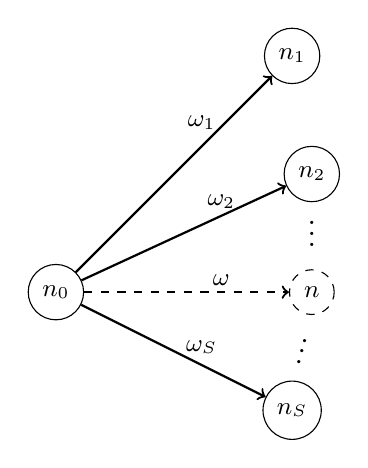
\begin{tikzpicture}

\draw (0,0) node(ROOT)[circle,draw]{\small $n_0$ };
\draw (3,3) node(ONE)[circle,draw]{ \small $n_1$ };
\draw (3.25,1.5) node(TWO)[circle,draw]{ \small $n_2$ };
\draw (3.25,.85) node(DOTONE){ \large $\vdots$ };
\draw (3.25,0) node(N)[circle,dashed,draw]{ \small $n$ };
\draw (3.15,-.65) node(DOTTWO)[rotate=-15]{ \large $\vdots$ };
\draw (3,-1.5) node(S)[circle,draw]{ \small $n_S$ };

\draw (1.85,2.15) node(OMG1){ \small $\omega_1$ };
\draw (2.1,1.15) node(OMG2){ \small $\omega_2$ };
\draw (2.1,.15) node(OMG){ \small $\omega$ };
\draw (1.85,-.7) node(OMGS){ \small $\omega_S$ };

\draw[thick, ->] (ROOT) -- (ONE) ;
\draw[thick,->] (ROOT) -- (TWO);
\draw[thick,dashed, ->] (ROOT) -- (N);
\draw[thick,->] (ROOT) -- (S);

%\draw[thick,dashed] (TWO) -- (N);
%\draw[thick,dashed] (N) -- (S);

\end{tikzpicture} 
\caption{Scenario Tree for Two Stage Problem}
  \label{fig:mip}
\end{figure}


\subsubsection{Finite Cycle Model}
The prior stochastic program is extremely greedy with regards to arbitrage opportunities and does not take into account the degradation from using cycles of the storage system.  Using $v$ as the value for a cycle of the storage system, the following penalty function is introduced.
\begin{equation}
	\lambda( x_n ) = \sum_t d_{nt} \left( \frac{v}{  \overline{E} - \underline{E} }\right)
\end{equation} 

Then, adding a penalty based on the value, (\ref{solve}) becomes the following.
\begin{subequations}
\begin{align}
	\mbox{ Maximize } \hspace{10px} & \pi_{n_0}(x_{n_0}) + \Expect_\Omega [ \pi_\omega(x_n) - \lambda(x_{n}) ]  & 	\\
	\mbox{ such that } \hspace{10px} & x_n \in \cX_{\omega_n}  & \forall \omega_n \in \Omega^S, n={n_1, \cdots, n_s}
\end{align}
\label{solvePenalty}
\end{subequations}



\subsubsection{Estimating Annual Effects}
Let $p_{i,weekday}, p_{i,weekend}, i = 1, \cdots, 4$ be the profits from arbitrage less the cost for travel found from solving stochastic program (\ref{solve}) or (\ref{solvePenalty}) for the various data sets.  Then a crude estimate of annual benefits $p$ and annual battery cycles $c$ can be found by the following.
\begin{align}
	p_n = \sum_{i=1}^4 13 [ 5 p_{i,weekday} + 2 p_{i,weekend} ]  \\
	c_n = \sum_{i=1}^4 13 [ 5 c_{i,weekday} + 2 c_{i,weekend} ]  
\end{align}

\subsubsection{Lifetime Benefits}
Using the number of annual cycles as well as the expected maximum cycles for the storage system, the lifetime $\tau$ can be estimated as $\tau = \frac{c_{max}}{c_n}$.  Then, for a given cost of capital $r$, the net present value of the arbitrage opportunity over its batteries lifetime can be found by the following.
\begin{equation}
	NPV = \sum_{n=1}^\tau \frac{p_n}{(1+r)^n}
\end{equation}

%
\begin{table}
\centering
\begin{tabular}{| l | c c | c c | c c |}
\hline
	&	\multicolumn{2}{  c | }{ Greedy Arbitrage } & \multicolumn{2}{  c |}{ Finite Cycles }  & \multicolumn{2}{  c |}{ Two Tier Rates} \\
	&	Model S 	& 	Leaf 	&	Model S 	& 	Leaf 	&	Model S 	& 	Leaf	\\
\hline
Annual Profit	&  	\$1014	&	\$235	&	\$744	&	\$173		&	\$2696		&	\$581	\\
Annual Cycles	&	585	&	476	&	218	&	176		&	233		&	164	\\
Value per Cycle&	1.73	&	0.49	&	3.4	&	0.98		&	11.57		&	3.54	\\
Battery Lifetime&	2	&	3	&	5	&	6		&	4		&	6	\\
NPV (r=5\%)	&	\$1886	&	\$640	&	\$3221	&	\$878		&	\$9559		&	\$2948	\\
\hline


\end{tabular}
\caption{Net Present Value (NPV) Calculation}
\end{table}



\subsubsection{Parameters for the Model}

\subsubsection{Madison, Wisconsin - Real Time Prices}
In order to investigate the costs and benefits of using electric vehicles for arbitrage, a local hypothetical example will be developed.  The user will have access to one of a variety of electric vehicles such as the Nissan Leaf or the Tesla Model S.  The user will be able to buy electricity from MG\&E at a fixed premium ($1+\gamma$) and sell electricty at market price.  Figure (\ref{fig:lmpweekday}) gives the pricing data for MG\&E Madison hub from MISO.  The example will be divided into 4 seasons, to get a rough estimation of the seasonal variation in price.    The user will be able to "plug-in" wherever convenient and still recieve payments for electricity sold to grid.  The user has a distribution of possible travel schedules for both the weekend and weekdays for all four seasons. 
\subimport{data/}{weekdays_plot}
%\subimport{data/}{weekend_plot}


\subsubsection{Vehicle Parameters}
In order for electric vehicles to be used for arbitrage, it will be critical to respect the user constraints.  This includes being able to use their car just like their traditional car as well as having the implementation be simple and straightforward.  The user constraints are primarly their particular vehicles characteristics, charging systems available, and a set of possible travel schedules which they may use.  Table (\ref{tab:evp}) shows the vehicle characteristics for several production vehicles as well as the Tesla Model S, which has not reached production stages as of yet.
\begin{table}
\centering
\begin{tabular}{| r |  c c |}
\hline
\rowcolor[gray]{.8} \bf Model		&	\bf Leaf  		&   \bf  Model S 	 \\
\hline
 Manufacturer 	&	Nissan		&	Tesla  	\\
\rowcolor[gray]{.95}Battery Size	&	24 kWh	&	85 kWh	\\
EPA Range	&	100 mi 		&	300 mi 		\\
\rowcolor[gray]{.95}Efficiency	&	.85		&	.9		\\
Charge		&	6.6 kW		&	20 kW		\\
\rowcolor[gray]{.95}Quick Charge	&	19.2 kW	&	80 kW		\\
Cost		&	\$ 35,200	&	\$69,900	\\
\rowcolor[gray]{.95}Expected Life	&	8 yr 		&	7r		\\
		&	100,000   	&	100,000 mi  	\\
\hline

\end{tabular}

\caption{ Electric Vehicle Parameters }
\label{tab:evp}
\end{table}

\subsubsection{Uncertain Travel Schedules}
The set of travel schedules represent the user's preferences when deciding the charging profile.  The charging profile will ensure that all of the possible travel schedules will not be restricted.  However, as more travel schedules are added, additional constraints are put on the charging profile.  This means that if one wanted an extremely flexible travel schedule, the charging plan is more restricted and less benefits from arbitrage are possible.  Additionally, a user may have substitutes available for travel.  For example, a bike, a bus, and a second car all represent secondary options for traveling to and from a destination.  The cost (direct and indirect) can be taken into account and a potentially lucrative arbitrage opportunity can be taken advantage of by using substitutes for travel.  Figure (\ref{fig:travel}) shows two examples of travel schedules. 

\begin{figure}
\centering

\subfigure[ Travel Schedule A ]{
\begin{tikzpicture}


\begin{axis}[ymin=0,ymax=30, xlabel=$Time$ (hour), ylabel=$Distance$ (miles), enlargelimits=false, width=12cm,height=3.5cm]
\addplot[const plot, pattern=flexible hatch,
        hatch distance=5pt,
        hatch thickness=0.5pt,
        pattern color=cyan, 
        draw=black]
coordinates
{ (0,0) 	(1, 0)  (2, 0) (3, 0) (4, 0) (5, 0) (6, 0) (7, 0) (7.5,18) (8.5, 0) 
   (10,0) (10.5, 4)  (11.5, 0) (13, 0) (14, 0) (15, 0) (16, 0) (16.5, 24) (17.5, 0) (18.5, 7) 
   (19.5,0) (21, 0)  (22, 0) (23, 0) (24, 0) } \closedcycle ;

\end{axis}

\end{tikzpicture}
}
\subfigure[ Travel Schedule B ]{
\begin{tikzpicture}


\begin{axis}[ymin=0,ymax=30, xlabel=$Time$ (hour), ylabel=$Distance$ (miles), enlargelimits=false, width=12cm,height=3.5cm]
\addplot[const plot, pattern=flexible hatch,
        hatch distance=5pt,
        hatch thickness=0.5pt,
        pattern color=cyan, 
        draw=black]
coordinates
{ (0,0) 	(1, 0)  (2, 0) (3, 0) (4, 0) (5, 0) (5.5, 12) (6.5, 0) (7.5, 20) (8.5, 0) 
   (10,0) (11, 0)  (12, 0) (13, 0) (14, 0) (15, 0) (15.5, 23) (16.5, 0) (18.5, 4) 
   (19.5,0) (21, 0)  (21.5, 7) (22.5, 0) (24, 0) } \closedcycle ;

\end{axis}

\end{tikzpicture}
}







\caption{Possible Travel Schedules}
\label{fig:travel}
\end{figure}

   

\subsubsection{Modeling in GAMS}
Using the algebraic modeling language GAMS, this stochastic program was described.  The parameters for the model were filled with data from electric vehicle table (\ref{tab:evp}) and pricing information in figure (\ref{fig:lmpweekday}).  Five travel schedules were generated and 15 different pricing scenarios were used, leading to 75 second stage nodes.  The model is solved under a minute and gives the charging profiles for all four seasons.  Figure (\ref{fig:eso}) shows the dispatch schedule for a Nissan Leaf and Tesla Model S for the February pricing information.  The model behaves as expected, storing energy while the prices are low and dispatching for arbitrage while the prices are high.  The Model S contains a large battery, so the amount need for travel is negligible.  It will be important to account for unavailability of car while driving in the next version of this model.

\pgfplotstableread
{./ex_modelS.dat}
{\loadedtable}

\begin{figure}
 \centering
\subfigure[  Tesla Model S with Large Battery System ]{
	\begin{tikzpicture}[scale=.8]
		\begin{axis}[xlabel=$Time$ (hour), ylabel=$Prices \hspace{7px} (\frac{\mbox{\$}}{\mbox{MWh}}$)
				%,scale only axis
				%,legend pos=outer north east 
				,width=12cm
				,axis y line*=left
				,extra y ticks={-50, 0, 50,100,150}
				,extra tick style={grid=major}
				,xmin=1,xmax=24
				,title=\mbox{\textbf{ Real Time Storage Operation }} ]

	
	\addplot+[opacity=.5, color=red,smooth,mark=o,line width=2pt] table[x=time, y=n0,mark=square] {./data/lmp_feb_3_2010.dat};
	\addlegendentry{Day Ahead Prices}
 	\addplot+[opacity=.5, smooth,solid,color=blue,mark=o,line width=2pt] table[x=time, y=n1] {./data/lmp_feb_3_2010.dat};
	\addlegendentry{Real Time Prices}
\foreach \i in {2,...,15}
{
 	\addplot+[opacity=.25, smooth,solid,color=black,mark=o] table[x=time, y=n\i] {./data/lmp_feb_3_2010.dat};
%	\addlegendentryexpanded{$n\i$}
}

		\end{axis}	
		
		\begin{axis}[xlabel=$t$ (hour), ylabel=$Energy \hspace{4px}$ (MW)
				%,ybar stacked
				%,scale only axis
				, const plot
				, stack plots=y
				, area style
				,width=12cm
				, axis y line=right
				, axis x line=none
				,xmin=1,xmax=24 
				,ymin=0,ymax=100
				,legend style={
					area legend,
					at={(0.5,-0.15)},
					anchor=north,
					legend columns=-1}]

 	\addplot+[%solid,color=black,
			%pattern=flexible hatch,
			%pattern color = cyan
			opacity=.75
			] table[x=time, y=e_r] from \loadedtable \closedcycle;
 	\addplot+[%color=red,
			%pattern=flexible hatch,
			%pattern color = red
			opacity=.75
			] table[x=time, y=s_r] from \loadedtable \closedcycle;
 	\addplot+[%color=red,
			%pattern=flexible hatch,
			%pattern color = red
			opacity=.75
			] table[x=time, y=d_r] from \loadedtable \closedcycle;
 	\addplot+[%color=red,
			%pattern=flexible hatch,
			%pattern color = red
			opacity=.75
			] table[x=time, y=t_r] from \loadedtable \closedcycle;
	\legend{Energy Level, Energy Stored, Energy Dispatched, Travel Energy}
 %	\addplot+[ybar, solid,color=black,
%			pattern=flexible hatch,
%			pattern color = green] table[x=time, y=sr] {./feb_ex_modelS.dat};
%	\addplot+ table[x=time, y=n0] { feb_ex_modelS.dat};		

		\end{axis}


	\end{tikzpicture}
}


\subfigure[  Nissan Leaf ]{
	\begin{tikzpicture}[scale=.8]
		\begin{axis}[xlabel=$Time$ (hour), ylabel=$Prices \hspace{7px} (\frac{\mbox{\$}}{\mbox{MWh}}$)
				%,scale only axis
				%,legend pos=outer north east 
				,width=12cm
				,axis y line*=left
				,extra y ticks={-50, 0, 50, 100,150}
				,extra tick style={grid=major}
				,xmin=1,xmax=24
				,title=\mbox{\textbf{ Real Time Storage Operation }} ]

	
	\addplot+[opacity=.5, color=red,smooth,mark=o,line width=2pt] table[x=time, y=n0,mark=square] {./data/lmp_feb_3_2010.dat};
	\addlegendentry{Day Ahead Prices}
 	\addplot+[opacity=.5, smooth,solid,color=blue,mark=o,line width=2pt] table[x=time, y=n1] {./data/lmp_feb_3_2010.dat};
	\addlegendentry{Real Time Prices}
\foreach \i in {2,...,15}
{
 	\addplot+[opacity=.25, smooth,solid,color=black,mark=o] table[x=time, y=n\i] {./data/lmp_feb_3_2010.dat};
%	\addlegendentryexpanded{$n\i$}
}

		\end{axis}	
		
		\begin{axis}[xlabel=$t$ (hour), ylabel=$Energy \hspace{4px}$ (MW)
				%,ybar stacked
				%,scale only axis
				, const plot
				, stack plots=y
				, area style
				,width=12cm
				, axis y line=right
				, axis x line=none
				,xmin=1,xmax=24 
				,ymin=0,ymax=30
				,legend style={
					area legend,
					at={(0.5,-0.15)},
					anchor=north,
					legend columns=-1}]

 	\addplot+[%solid,color=black,
			%pattern=flexible hatch,
			%pattern color = cyan
			opacity=.75
			] table[x=time, y=e_r] {feb_ex_leaf.dat} \closedcycle;
 	\addplot+[%color=red,
			%pattern=flexible hatch,
			%pattern color = red
			opacity=.75
			] table[x=time, y=s_r] {feb_ex_leaf.dat} \closedcycle;
 	\addplot+[%color=red,
			%pattern=flexible hatch,
			%pattern color = red
			opacity=.75
			] table[x=time, y=d_r] {feb_ex_leaf.dat} \closedcycle;
 	\addplot+[%color=red,
			%pattern=flexible hatch,
			%pattern color = red
			opacity=.75
			] table[x=time, y=t_r] {feb_ex_leaf.dat} \closedcycle;
	\legend{Energy Level, Energy Stored, Energy Dispatched, Travel Energy}
 %	\addplot+[ybar, solid,color=black,
%			pattern=flexible hatch,
%			pattern color = green] table[x=time, y=sr] {./feb_ex_modelS.dat};
%	\addplot+ table[x=time, y=n0] { feb_ex_modelS.dat};		

		\end{axis}


	\end{tikzpicture}
}



  \caption{Energy Storage Operation }
 \label{fig:eso}
\end{figure}


\subsubsection{Example of Model Results}
The model is solved for the four seasons twice, once allowing for arbitrage, and a second not allowing arbitrage to find the cost of operating the car for travel alone.  The value of the arbitrage opportunity is the benefits allowing arbitrage less the benefits with no arbitrage.  The results for the two cars are shown in table (\ref{tab:res}).  Along with the profits from operation, the number of cycles the battery undergoes is accounted for.


\begin{table}[ht]
\centering
\subtable[ Tesla Model S results ]{
\begin{tabular}{| c | c c | }
\hline
\multicolumn{3}{ | c |  }{ Daily Cost, Benefit (Dollars) } \\
\hline
\bf Model S &    Arbitrage    &      No Arbitrage \\
\hline
Season 1     &   1.238     & -1.740	\\
Season 2     &  1.496     & -1.109	\\
Season 3     & 2.031     & -1.603	\\
Season 4     & 1.663    &  -0.697	\\
\hline
\end{tabular}

\begin{tabular}{| c | c c | }
\hline
\multicolumn{3}{ | c |  }{ Daily Cycles } \\
\hline
\bf Model S &    Arbitrage    &      No Arbitrage \\
\hline
Season 1 &      2.110  &     0.174\\
Season 2 &       1.752  &     0.174\\
Season 3 &       1.533   &    0.174\\
Season 4 &       1.732    &   0.174	\\
\hline
\end{tabular}
}

\subtable[ Nissan Leaf results]{

\begin{tabular}{| c | c c | }
\hline
\multicolumn{3}{ | c |  }{ Daily Cost, Benefit (Dollars) } \\
\hline
\bf Leaf &    Arbitrage    &      No Arbitrage \\
\hline
Season 1   &    0.066  &    -0.661	\\
Season 2   &    0.205  &    -0.422	\\
Season 3   &    0.252  &    -0.581	\\
Season 4  &     0.324  &    -0.179	\\

\hline
\end{tabular}

\begin{tabular}{| c | c c | }
\hline
\multicolumn{3}{ | c |  }{ Daily Cycles } \\
\hline
\bf Leaf &    Arbitrage    &      No Arbitrage \\
\hline
Season 1   &    2.106  &     0.562	\\
Season 2   &    1.831  &     0.562	\\
Season 3   &    1.590  &     0.562	\\	
Season 4   &    1.759  &     0.562		\\

\hline
\end{tabular}
}
\caption{Results from Arbitrage Model}
\label{tab:res}
\end{table}
%
\begin{table}[ht]
\centering
\subtable[ Tesla Model S results ]{
\begin{tabular}{| c | c c | }
\hline
\multicolumn{3}{ | c |  }{ Daily Cost, Benefit (Dollars) } \\
\hline
\bf Model S &    Arbitrage    &      No Arbitrage \\
\hline
Season 1     &   .944     & -1.632	\\
Season 2     &  .738     & -1.899	\\
Season 3     & 1.034     & -1.178	\\
Season 4     & 1.457    &  -1.186	\\
\hline
\end{tabular}

\begin{tabular}{| c | c c | }
\hline
\multicolumn{3}{ | c |  }{ Daily Cycles } \\
\hline
\bf Model S &    Arbitrage    &      No Arbitrage \\
\hline
Season 1 &      2.049  &     0.099\\
Season 2 &       1.598  &     0.099\\
Season 3 &       1.356   &    0.099\\
Season 4 &       1.821    &   0.099	\\
\hline
\end{tabular}
}

\subtable[ Nissan Leaf results]{

\begin{tabular}{| c | c c | }
\hline
\multicolumn{3}{ | c |  }{ Daily Cost, Benefit (Dollars) } \\
\hline
\bf Leaf &    Arbitrage    &      No Arbitrage \\
\hline
Season 1   &    0.203  &    -0.527	\\
Season 2   &    0.156  &    -0.219	\\
Season 3   &    0.200  &    -0.324	\\
Season 4  &     0.435  &    -0.250	\\

\hline
\end{tabular}

\begin{tabular}{| c | c c | }
\hline
\multicolumn{3}{ | c |  }{ Daily Cycles } \\
\hline
\bf Leaf &    Arbitrage    &      No Arbitrage \\
\hline
Season 1   &    2.116  &     0.322	\\
Season 2   &    1.719  &     0.322	\\
Season 3   &    1.399  &     0.322	\\	
Season 4   &    1.793  &     0.322		\\

\hline
\end{tabular}
}
\caption{Results from Arbitrage Model}
\label{tab:resWE}
\end{table}

\subsubsection{References}
\begin{itemize}
\item \url{http://www1.eere.energy.gov/femp/pdfs/primer.pdf}\\
\item \url{http://eetd.lbl.gov/ea/EMP/reports/54238.pdf}\\
\item \url{http://www.beg.utexas.edu/energyecon/new-era/case_studies/Electricity_Restructuring_in_California.pdf}\\
%\mbox{miso monthly markets and operation reports december 2011}\\
\item \url{https://www.midwestiso.org/Library/Repository/Meeting\%20Material/Stakeholder/BOD/Markets\%20Committee/2012/20120118/20120118\%20Markets\%20Committee\%20of\%20the\%20BOD\%20Item\%2004\%20Markets\%20and\%20Operations\%20Report.pdf}
\item \url{http://web.mit.edu/sloan-auto-lab/research/beforeh2/files/PHEV\%20costs.pdf}\\
\item \url{http://www.mge.com/home/rates/residential_elec.htm#RG-2}
\item \url{http://www.mge.com/images/PDF/Electric/Rates/E07.pdf}
\end{itemize}


%\begin{figure}
\centering
	\subfigure[Day Ahead Market]{ \label{fig:dam}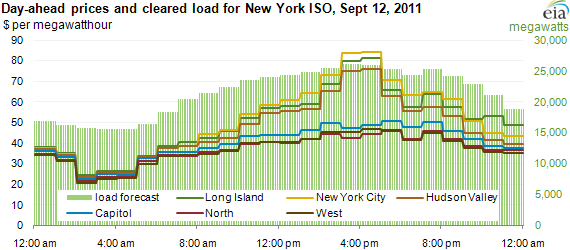
\includegraphics[width=4in, clip=18px 0 0 0]{ferc_day_ahead} }
	\subfigure[Real Time Market]{ \label{fig:rtm}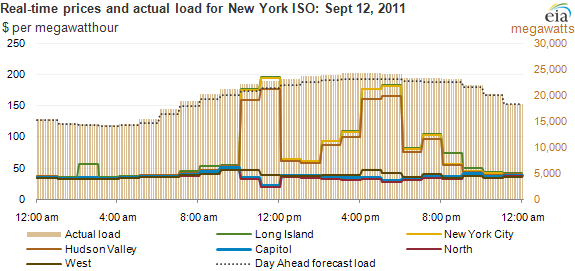
\includegraphics[width=4in]{ferc_real_time} }
\caption{Electricity Markets}
  \label{fig:em}
\end{figure}

%weekdays
%\subimport{data/}{feb3_plot}
%\subimport{data/}{may5_plot}
%\subimport{data/}{aug4_plot}
%\subimport{data/}{nov3_plot}

%weekends
%\subimport{data/}{feb6_plot}
%\subimport{data/}{may8_plot}
%\subimport{data/}{aug7_plot}
%\subimport{data/}{nov6_plot}


%\subimport{data/}{aug4_table}
